\documentclass[a4paper]{iacas}

\usepackage{cite}
\usepackage{hyperref}% embedding hyperlinks [must be loaded after dropping]
\usepackage{amsmath,amsthm,amssymb,amsfonts,latexsym,mathrsfs,wasysym}
\usepackage{marvosym}
\usepackage{subcaption}
\usepackage{soul,color}
\usepackage{threeparttable}% tables with footnotes
\usepackage{dcolumn}% decimal-aligned tabular math columns
\usepackage{float}
\usepackage{graphicx}
%\usepackage{accents}
\usepackage{tikz}
\usepackage{lastpage}
\usepackage{fancyhdr}
\usepackage{color}
\usepackage{cancel}
\usepackage{setspace}
\usepackage{physics}
\usepackage{enumitem}
\usepackage{graphicx}

	% use for derivatives:
%	\dv{Q}{t} = \dv{s}{t}  \quad
%	\dv[n]{Q}{t} = \dv[n]{s}{t}  \quad
%	\pdv{Q}{t} = \pdv{s}{t}  \quad
%	\pdv[n]{Q}{t} = \pdv[n]{s}{t}  \quad
%	\pdv{Q}{x}{t} = \pdv{s}{x}{t}  \quad

%\doublespacing
% or:
\onehalfspacing
%\usepackage[T1]{fontenc}
%\usepackage{bigfoot} % to allow verbatim in footnote
\usepackage[framed,numbered]{matlab-prettifier}
\pagestyle{plain}
%\usepackage[hebrew,english]{babel}
\usetikzlibrary{shapes.geometric, arrows, calc}

\newcolumntype{d}{D{.}{.}{-1}}
\graphicspath{{figures/}}

% define some commands to maintain consistency
\newcommand{\pkg}[1]{\texttt{#1}}
\newcommand{\cls}[1]{\textsf{#1}}
\newcommand{\file}[1]{\texttt{#1}}
\newcommand{\sgn}[1]{\operatorname{sgn}\left(#1\right)}
\newcommand{\sat}[1]{\operatorname{sat}\left(#1\right)}
\newcommand{\rrule}[1]{\rule[#1]{0pt}{0pt}}
\newcommand{\fracds}[2]{\frac{\displaystyle #1\rrule{-0.2em}}{\displaystyle #2\rrule{1em}}}
\newcommand{\figref}[1]{Fig.~\ref{#1}}
\newcommand{\ubar}[1]{\underaccent{\bar}{#1}}
%	\newcommand{\norm}[1]{\lvert \lvert \vec #1 \rvert \rvert}


%diffeomorphism

% XeLaTeX!
% ============================================================ %
% HEBREW support via polyglossia %
% ============================================================ %
	\usepackage{polyglossia}
	\defaultfontfeatures{Mapping=tex-text, Scale=MatchLowercase}
	\setdefaultlanguage{english}
	\setotherlanguage{hebrew}
	\newfontfamily\hebrewfont[Script=Hebrew]{Times New Roman}
% Use \begin{hebrew} block of text \end{hebrew} for paragraphs.
% Use \texthebrew{ } and \textenglish{ } for short texts.
% ============================================================ %



\begin{document}

\begin{center}
 \large Image processing - 046200
 \end{center}
\begin{center}
\large\textbf{Homework \#3}
 \end{center}


\begin{tabular}{l}
\\
{\bf\textit{Alexander Shender 328626114}} \\
{\bf\textit{Sahar Carmel 305554453}} \\
Technion - Israel Institute of Technology
\end{tabular}

\vspace{2em}

\newpage


\begin{hebrew}
\textit{\huge שאלה 1.}

א. ניתן לראות שהפעולה שאנו מבצעים הינה פעולת קונבולוציה עם דלתא של הזזה שמוגדרת כ: 
\end{hebrew}
$\delta(m-m_i,n-n_i)$
\begin{hebrew}
ולכן אנו נוכל לרשום את התמונה של $X[m,n]$ כסכום של קונבולוציות:
\end{hebrew}
$$X[m,n]  =\sum^P_{x=1}\phi[m,n]*\delta(m-m_i,n-n_i) \Longrightarrow h[m,n] = \delta(m-m_i,n-n_i)$$

\begin{hebrew}

ב. הזזה הינה אכן פעולה ספרבילית, כי ניתן לפרק את התזוזה לציר $X$ וגם לציר $Y$. נרחיב את הביטוי שמצאנו, לפירוק לשני הצירים:
\end{hebrew}
$$X[m,n]  =\sum^P_{x=1}\phi[m,n]*\delta(m-m_i,n-n_i) = \sum^P_{x=1}\phi[m,n]*(\delta(m-m_i)\delta(n-n_i))$$
\begin{hebrew}
ג. בדרך כלל, כנגד ה-$salt \& pepper$ השיטה המועילה להתגבר עליה הינה המסנן החציון. אך במקרה שלנו זאת לא השיטה שתניב תוצאה סבירה:
\\בהנחה שהתמונות $\psi[m,n]$ מפוזרות מספיק רחב בתמונה אנו נקבל שמסנן חציון יאפס לנו את כל התמונה (אלא אם כן יצא מקרה דופק בו נקבל 5 פיקסלים עם ערך 1 בריבוע של 9 פיקסלים, מה שאינו סביר, כי רק $3\%$ מהפיקסלים הם מרועשים).
\\בהנחה שהתמונות $\psi[m,n]$ מפורזרות מאד צפוף, נקבל שפיקסלים שבמקור היו לבנים, יקבלו עכשיו ערכים. וזה לא רצוי.
\end{hebrew}
\newline
\begin{hebrew}
השיטה המועילה לדעתינו תהיה השיטה של $\textrm{template matching}$. כתבנית אנו נשתמש בתמונה $\psi[m,n]$ , ובמקום בו אנו נקבל התאמה מעל סף מסוים שנקבע, נכניס את התמונה  $\psi[m,n]$ בתמונה החדשה שנגדיר. ככה נקרב את התנונה $\hat{U}[m,n]$ לתמונה המקורית האמיתית $U[m,n]$ 
\end{hebrew}


\newpage
\begin{hebrew}
\textit{\huge שאלה 2.}

א. נמצא את הסינון הלינארי. נתבונן רק בפילטר של השחזור, ונמצא פילטר בודד:
\end{hebrew}
\begin{equation*}
\alpha(1+k\nabla^2) = \alpha\left(\begin{bmatrix}0&0&0\\0&1&0\\0&0&0\end{bmatrix}+K\begin{bmatrix}0&1&0\\1&-4&1\\0&1&0\end{bmatrix}\right) = \begin{bmatrix}0&K&0\\K&\alpha-4K&K\\0&K&0\end{bmatrix}
\end{equation*}
\begin{hebrew}
כעת, על מנת לקבל סינון לינארי שעוברת התמונה, נשתמש גם במודל טשטוש שהוצע. נבצע קונבולוציה:
\end{hebrew}
\begin{equation*}
\psi = \frac{1}{8}\cdot \begin{bmatrix}0&K&0\\K&\alpha-4K&K\\0&K&0\end{bmatrix} * \begin{bmatrix}0&1&0\\1&4&1\\0&1&0\end{bmatrix}  = \frac{1}{8} \cdot \begin{bmatrix}0&0&K&0&0\\0&2K&\alpha&2K&0\\K&\alpha&4\alpha-12K&\alpha&K\\0&2K&\alpha&2K&0\\0&0&K&0&0\end{bmatrix}
\end{equation*}

\begin{hebrew}
ב. נמצא את $\alpha$ שישמור על הממוצע של התמונה המקורית. לטובת זאת, נשווה את הממוצע של הפילטר ל-1:
\end{hebrew}

\begin{equation*}
mean = \frac{1}{8} \cdot (12\cdot K + 8\cdot\alpha - 12K) = 1  \Longrightarrow  \alpha = \frac{8}{8} = 1
\end{equation*}

\begin{hebrew}
ג. כעת נתון ש-$\alpha$ הינו 1. כמו כן, מצאנו שגרעין $\psi$ הינו $5X5$, כלומר $M=N=5$ נמצא את K אשר ימזער את השגיאה הריבועית המוגדרת:
\end{hebrew}
\begin{equation*}
E = \sum_{m=1}^M \sum_{m=1}^M |\psi -\delta|^2
\end{equation*}
\begin{equation*}
\psi -\delta  = \begin{bmatrix}0&0&K&0&0\\0&2K&1&2K&0\\K&1&3-12K&1&K\\0&2K&1&2K&0\\0&0&K&0&0\end{bmatrix}
\end{equation*}
\begin{equation*}
E = |\psi -\delta|^2 = 4\cdot K^2 + 4\cdot (2K)^2 + 4 + (3-12K)^2
\end{equation*}
\begin{hebrew}
נמצא את המינימום, נגזור, נשווה ל-0
\end{hebrew}
\begin{equation*}
\frac{\partial E}{\partial K} = \frac{\partial{|\psi -\delta|^2}}{\partial K} = 8K + 16K + 2(3-12K) = 24K -24K + 6 = 0
\end{equation*}
\begin{equation*}
\Longrightarrow 6 = 0 (???)
\end{equation*}


\newpage

\begin{hebrew}
\textit{\huge שאלה 2.}

א. נמצא אלמנט בנייה עבור כל אחת מהתמונות $a-d$:
\end{hebrew}

For each case, we put the element onto the original figure to indicate the proportion

\begin{enumerate}[label=(\alph*.)]

\item The operation is \textbf{erosion}, the structuring element is the following, where C indicates the center
\newline
\newline
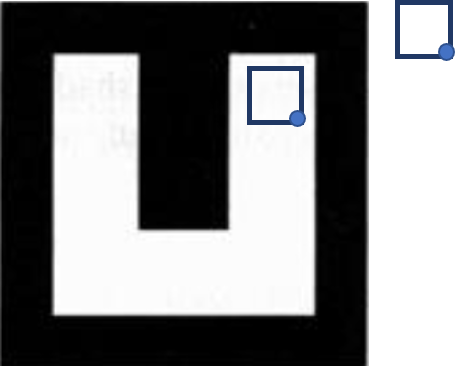
\includegraphics{imgs/q3_11.png}
\item The operation is \textbf{erosion}, the structuring element is the following, where C indicates the center
\newline
\newline
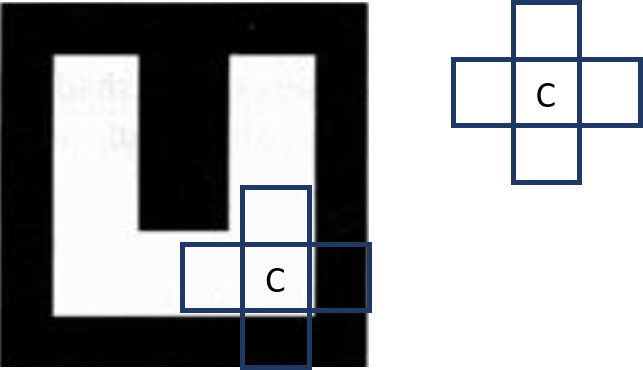
\includegraphics{imgs/q3_12.png}
\item The operation is \textbf{erosion}, the structuring element is the following, where the dot indicates the center. Notice that the upper and lower parts in the structuring element were added so that the "connecting" part in the "U" shape will have overlap with some of surrounding black part, thus resulting in '0'.
\newline
\newline
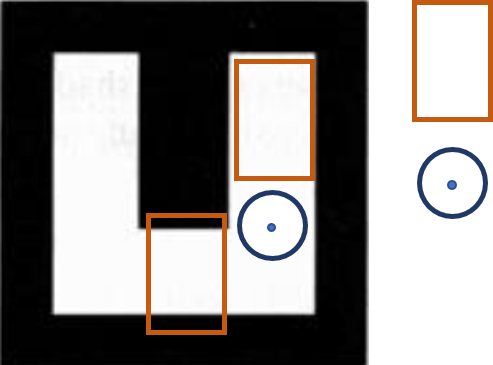
\includegraphics{imgs/q3_13.png}
\item The operation is \textbf{dilation}, the structuring element is the following, where the dot indicates the center.
\newline
\newline
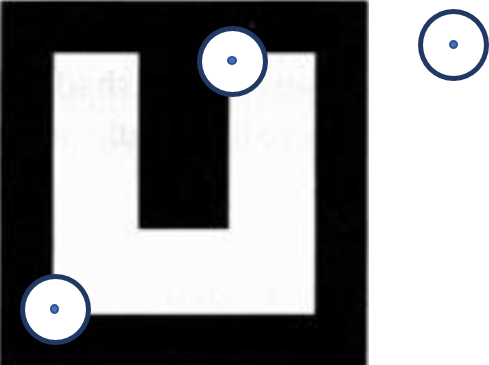
\includegraphics{imgs/q3_14.png}


\end{enumerate}


\begin{hebrew}
ב. התשובות הן להלן:
\end{hebrew}











\end{document}





